
% book - Default class for a normal book
\documentclass[a4paper,12pt,oneside]{book}

%textbook - a class for text bigger than 12pt
%\documentclass[a4paper,14pt,twoside,openright,reqno,table]{extbook}

% Options in detail:
% openany - allows chapter and similar openings to occur on left hand pages
% openright - allows chapter and similar openings tohttps://www.overleaf.com/project/620273a89e158f6264034920 occur on right hand pages
% fleqn  - left-alignment of formulas
% leqno - labels formulas on the left-hand side instead of right
% reqno - labels formulas on the right-hand side
% draft - in draft mode the figures are not loaded, useful for speeding up typesetting
% onecolumn or twocolumn
% oneside (default for article and report)
% twoside (default for book)
% table  --> to avoid the message: package xcolor has already been loaded ...
\usepackage{packages}
\usepackage{csquotes}
% Almost all the settings are defined in packages.sty

% Put a grey textual watermark on document pages (PS mode only)
%\usepackage[italian,light,first,bottomafter]{draftcopy}

% Put a grey textual watermark on document pages (PDF mode)
%\usepackage{draftwatermark}
% If you want to change the default DRAFT text
%\SetWatermarkText{DRAFT}
% If you want to change the default grey color of the text
%\SetWatermarkColor{red}

%%%%%%%%%%%%%%%%%%%%%%%%%%%%%%%%%%%%%%%%%%%
%   DOCUMENT: an ordered list of files    %
%             that you can include or not %
%             in your document            %
%%%%%%%%%%%%%%%%%%%%%%%%%%%%%%%%%%%%%%%%%%%
\begin{document}


% Title Page %
% ====================== Centred Title Page ===========================

% \begin{titlepage}
% \thispagestyle{empty}
% \centering
% %\providecommand\pdfbookmark[3][]{} \pdfbookmark[0]{Title Page}{bm:Title}
% \vspace*{5cm}
% \textsc{\huge{First Line of Your Title}}\\[0.5em]
% \textsc{\huge{Second Line}}\\[0.5em]
% \textsc{\huge{Third}}\\[0.5em]
% \vfill
% By\\[0.5em]
% \textsc{\Large{Joseph Chamberlain}}
% \vfill
% A thesis submitted to\\[-0.8em]
% the University of Birmingham\\[-0.8em]
% for the  degree of\\[-0.8em]
% \MakeUppercase{Doctor of Philosophy} \\[\baselineskip]
% \begin{figure}[ht!]
% \begin{center}
% 
\includegraphics[height=4cm]{frontmatter/images/BirminghamUniversityCrest.png}
% \end{center}
% \end{figure}
% Cold Atoms Research Group\\[-0.8em]
% School of Physics and Astronomy\\[-0.8em]
% College of Engineering and Physical Sciences\\[-0.8em]
% University of Birmingham\\[-0.8em]
% September~2020 \\[\baselineskip]
% %\copyright\ Copyright by \MakeUppercase{\@Author},~\@Year\\
% %All Rights Reserved
% \end{titlepage}
% \clearpage

% ================ Aligned Title Page ===========================

\thispagestyle{empty}
\providecommand\pdfbookmark[3][]{} \pdfbookmark[0]{Title Page}{bm:Title}
\vspace*{1cm}
\begin{figure}[ht!]

\includegraphics[height=4cm]{frontmatter/images/BirminghamUniversityCrest.png}
\end{figure}
\vfill
\begin{flushleft}
\textsc{\huge{Tackling internet inefficiency }}\\[0.5em]
\textsc{\huge{in modern-day}}\\[0.5em]
\textsc{\huge{Attendance monitoring Systems}}\\[0.5em]
\vfill
By\\[\baselineskip]
\textsc{\Large{Victor Nyoyoko}}
\vfill
1961453\\[-0.8em]
MEng Computer Science / Software Engineering FT\\[-0.8em]
\vfill
supervised by\\[-0.8em]
\vfill
\MakeUppercase{AHMAD IBRAHIM} \\[\baselineskip]
\end{flushleft}
\begin{flushright}
School of Computer Science\\[-0.8em]
College of Engineering and Physical Sciences\\[-0.8em]
University of Birmingham\\[-0.8em]
September~2021 \\[\baselineskip]
\end{flushright}
\copyright\ Copyright by \MakeUppercase{\@Nyoyoko Victor},~\@2022\\
%All Rights Reserved
\clearpage
%your name
%studentID
%programme name
% supervisor's name
% word count
%% FRONTMATTER %%
% The pages inside of frontmatter are in Roman numerals and the chapters will not have numeration
\frontmatter

% COPYRIGHT %
%% ======================== Copyright page ===============================

\thispagestyle{empty}
%\providecommand\pdfbookmark[3][]{} \pdfbookmark[0]{Copyright}{bm:Copyright}
\addtocounter{page}{-1}
\vspace*{\fill}
\vfill
\begin{center}
\copyright\ Copyright by \MakeUppercase{Joseph Chamberlain},~2020\\
All Rights Reserved
\end{center}
%\vspace{1in}
\clearpage

% ABSTRACT %
\providecommand\phantomsection{} \phantomsection
%\addcontentsline{toc}{part}{Abstract}
\begin{center}
%\hrule
\providecommand\pdfbookmark[3][]{} \pdfbookmark[0]{Abstract}{bm:Abstract}
\vspace*{1in}
\textbf{ABSTRACT}\\[2\baselineskip]
% \vspace*{.1in}
\end{center}

(problems)
For over four years in the University of Birmingham campus, I  have taken note of the attendance monitoring system, the inefficiency in tracking attendance in a Wide Area Network and it's causes, due to the number of users and the range (even with the boosters) of connectivity, Usually attendance in Birmingham is answered on canvas in a quiz form. Most of the time 
we can't access the internet and if we(users) don't have data we are unable to track. This prevents the 
university from tracking Lecture activities in the school.. There are more places like this with this inability to have a reliable internet connection and have issues with tracking attendance in monitoring system. I decided to develop an attendance system with a raspberry pi, a website, RFID and a Fingerprint module with Azure Cloud Computing Service where I designed and implemented a database and internet exception handler for this system that stores attendance data temporarily on the raspberry pi and sends it later on when there's internet access. This produced a system that is capable of tracking attendance in cases of short internet latency gaps given different options and tracking choices. It seems to curb the problems of not connecting to database by storing data temporarily on the raspberry-pi and sending it back up when the internet is on.

Being tested with large set of data this seems to fix 
\textbf{}





% DEDICATION %
% % ======================= Dedication Page ============================
\newpage
\thispagestyle{plain}%
\begin{center}
%\providecommand\pdfbookmark[3][]{}\pdfbookmark[0]{DedicationPage}{bm:Dedicate}
\vspace*{1.575in}
\textbf{DEDICATION}\\[2\baselineskip]
Dedicated to my cats
\end{center}%
\vfill
\newpage


% ACKNOWLEDGEMENTS %
% % ========================= Acknowledgments ==============================
\providecommand\phantomsection{} \phantomsection
%\addcontentsline{toc}{part}{Acknowledgments}
\thispagestyle{plain}
\renewcommand{\baselinestretch}{1}\small\normalsize
\begin{center}
%\providecommand\pdfbookmark[3][]{}\pdfbookmark[0]{Acknowledgments}{bm:Acknowledge}
\vspace*{0.375in}
\textbf{ACKNOWLEDGMENTS}\\[3\baselineskip]
\end{center}
\renewcommand{\baselinestretch}{1.66} \small\normalsize%
I acknowledge the people who helped me.
\newpage

% CREDITS %
% \begin{titlepage}

\nonumber
\null \vspace {\stretch{1}}
%	\begin{flushright}
%	\begin{verse}
    \begin{center}
\textit{Worker bees can leave\\
even drones can leave\\
the queen is their slave} \\[5mm]
%	\end{verse}
	Tyler Durden, ''Fight Club''
%	\end{flushright}
    \end{center}
\vspace{\stretch{2}}\null

\end{titlepage}
\cleardoublepage

% CONTENTS %
% % To help hyperref to jump to the correct page
\phantomsection
%\addcontentsline{toc}{chapter}{Contents}
\tableofcontents

\renewcommand{\cftpartfont}{\normalfont\bfseries} % \part font in ToC
\renewcommand{\cftchapfont}{\normalfont\bfseries} % \chapter font in ToC
\renewcommand{\cftchappagefont}{\normalfont}
\renewcommand{\cftpartpagefont}{\normalfont}
\renewcommand{\cftpartleader}{\cftdotfill{\cftdotsep}}
\renewcommand{\cftchapleader}{\cftdotfill{\cftdotsep}}
\renewcommand{\cftsecleader}{\cftdotfill{\cftdotsep}}
% \setcounter{tocdepth}{4}
% \setcounter{secnumdepth}{4}

\cftsetindents{chapter}{0in}{0.25in}
\cftsetindents{section}{0.25in}{0.35in}
\cftsetindents{subsection}{.6in}{0.5in}
\cftsetindents{subsubsection}{1.5in}{0.5in}

\setlength{\cftbeforepartskip}{.25em}
\setlength{\cftbeforechapskip}{.25em}
\setlength{\cftbeforesecskip}{-.5em}
\setlength{\cftbeforesubsecskip}{-.5em}

\addtocontents{toc}{~\hfill\textbf{Page}\par}
\thispagestyle{plain}

\clearpage

  % Make the list of figures
\listoffigures
\thispagestyle{plain}
\clearpage

 % Make the list of tables
\listoftables
\thispagestyle{plain}
\clearpage
 



% GLOSSARY %
\cleardoublepage
% To help hyperref to jump to the correct page
\phantomsection
% To add the Glossary in the table of contents
%\addcontentsline{toc}{chapter}{Glossary}
% Prints the glossary
\printglossary

% In order to update the glossary you have to execute:
% \makeindex -s main.ist -t main.alg -o main.acr main.acn
% to insert an item in the document:
% \newglossaryentry{item_label}{name={item}, description={description}}
% if it doesn't appear you have to initialize it:
% \glsadd{item_label}
% or if it is called again in the following text:
% \gls{item_label}

% ACRONYMS %
\cleardoublepage
% To help hyperref to jump to the correct page
\phantomsection
% To add the Index of Symbols in the table of contents
%\addcontentsline{toc}{chapter}{Acronyms}
% Prints the Acronyms
\printglossary[type=\acronymtype,title=Acronyms]

% In order to update the symbols you have to execute:
% makeindex -s main.ist -t main.glg -o main.gls main.glo
% to insert an item in the document::
% \newacronym{item_label}{name={item}, description={description}}
% if it doesn't appear you have to initialize it:
% \glsadd{item_label}
% or if it is called again in the following text:
% \gls{item_label}

%% MAINMATTER %%
% The pages inside of mainmatter are in Arabic numerals and the chapters will have numeration
\mainmatter

%\part{If you want parts}
\chapter{Introduction}
Right from the moment we(humans) discovered the need to keep track of attendance in different environments, automation, accuracy and reliability have been the principle. In as much as we have Attendance Monitoring Systems which efficiently do their jobs,there are places where there are unreliable internet connectivity, caused by many external factors like latency, packet loss. This project investigates through the field of IoT to find a solution that solves this problem.


\section{Project Aims}

The aim of this project is to build a attendance monitoring system that is able to track attendance with a diverse number of methods while also being able to this with unreliable internet connectivity. 

The main evaluation criteria
\newacronym{IoT}{$IoT$}{Internet of Things}
\glsadd{IoT}

\newacronym{RFID}{$RFID$}{Radio-Frequency Identification}
\glsadd{RFID}

\section{Related Works} 
These are ways most authors have used to solve the issue of inefficiency in attendance monitoring systems.
\subsection{General texts}
The authors think it is a waste of time monitoring both body temperature and attendance in schools which is a problem caused by the COVID-19 pandemic, and seeks to join these two systems to monitor attendance as well as monitor body status and store the data to be accessed remotely across the globe\cite{KaziARP}. This influenced the merging of multiple attendance methods in my work.
The author proposed a smart attendance to evade the use of manual attendance system and reduce manual work of teachers and administrators, by building a system that monitors attendance with passive RFID and sends the data attained to the Cloud.
The authors seek to create a fast, automated, reliable and accurate system that monitors attendance by reading tags in the lecture room using an Ultra-High frequency reader and a middleware to sort, convert and relay data to the database system\cite{Www2012}. 
The author proposes a system that effectively and efficiently monitors attendance monitors with a website and RFID reader using an MQTT protocol and a NodeMCU firmware with the aim of eradicating manual attendance saving cost\cite{Bhagat2020}.
The author proposes fingerprint based biometric attendance system that monitors attendance and prevents giving proxy i.e when someone scans attendance for someone else, the data is stored in an SD card and later extracted. 

The author seeks to solve student performance by designing an efficient algorithm that detects and 


\subsubsection{Theoretical Approaches}
With the currently existing projects and literature in this field, a lot of the authors centralize on the inefficiency of attendance monitoring system based on the previous methods used and devise new methods as a solution[1,2 and more]. 

\subsubsection{Empirical Research}
[2] talks about the reliability and security of a system to prohibit truancy and develops a solution to stop it, Fingerprint is used as a tracking method because it's more reliable, accurate and cost effective (explain) and a GSM to alert guardians, if a student doesn't attend.

A limitation of this solution, it's not automated, teacher or an authorized has to get SD card from micro controller to store attendance in database.


\subsection{Central texts}

In as much as efficiency is quite the central theme in these literatures, I see only one solution being applied in these literatures and that has to do with using a more efficient method, why not use multiple methods for different scenarios, in some cases some methods might be more efficient in taking attendance and having them integrated makes the system flexible and better or even more efficient(in theory) in tracking attendance.

In "An Investigation on the viability of using IoT for student survey and attendance monitoring"[4]



A solution of mine was gotten from [3],which stores a temporary file directory before being sent to the database.

\chapter{Background}
The system is split into three different parts, the website, raspberry pi and the cloud(Azure), these are also split in their respective parts with website containing the web server(node) and the site(React), the Cloud; 
\begin{itemize}
  \item Azure sql server
  \item Azure sql database
\end{itemize}
\section{Website}
A website is often confused with a webpage or a web server. From mozillaWebDoc, A website is a collection of web pages which are grouped together in various ways. A web server hosts websites and their supporting files are available on the that computer. 
How do they talk to each other?
A website talks to the web server using an API, which is a connection between to computer programs. It could be referred also as the specification or as the implementation, the specification has to do with a document that demonstrates how to use or create a connection. Examples of API specifications used in this project are; tedious for the database connection to azure, express as a middleware. 

\newacronym{API}{$API$}{Application Programming Interface}
\glsadd{API}

\section{Raspberry-pi}
A portable computer with 40 GPIO pins, 
GPIO is an uncommitted digital pin on an electronic circuit board which may be used as input or output or both, and can be configured by the user at runtime[6]. This GPIO allows to interface with different modules. A module here is a small unit that can be integrated into a larger system but also maintained separately with no effect on the system. It is of a "plug-in" functionality.
To connect to azure from the raspberry pi, "pyodbc" driver is used. The driver files are installed on the raspberry-pi
LED  

\newacronym{GPIO}{$GPIO$}{General Purpose Input Output}
\glsadd{GPIO}

\subsection{RFID - RC522}
\subsubsection{Interfacing with the Rasberry pi}
The RFID card interfaces with the raspberry-pi with SPI communication but is also compatible with 1\textsuperscript{2}C and UART communication, it is a synchronous serial communication that encourages communication over a short distance, it is mainly used in embedded systems. Serial communication has to do with sending one bit at a time sequentially and synchronous means that this communication is synchronized by a clock signal which is used orchestrate the actions of the digital circuit i.e to determine when it is time to read the next bit/value. SPI devices communicate in a full duplex mode with a master-slave principle normally with a single master. full duplex means that data is transmitted back and forth simultaneously in this communication channel.

\textit{Note: The master is the raspberry pi.}
\vspace{1cm}
\begin{figure}[h]
  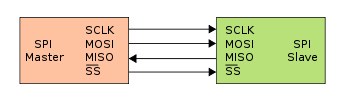
\includegraphics{Background/images/350px-SPI_single_slave.svg.png.png}
  \caption{SPI master slave architecture}
\end{figure}

\newacronym{1\textsuperscript{2}C}{$12C$}{Inter-Integrated Circuit}
\glsadd{12C}
\newacronym{SPI}{$SPI$}{Serial Peripheral Interface}
\glsadd{SPI}
SPI has four main logic signals: 
\begin{itemize}
  \item SCLK: Serial clock, which accepts pulses obtained from the master
  \item MOSI: Master Out Slave In, this is data transmitted from the master to slave
  \item MISO: Master In Slave Out, this is data transmitted from the slave to master
  \item CS/SS: Chip/Slave Select, an output from the master to notify data is being transmitted.
\end{itemize}

The RC522 module has 8 pins that interfaces with the raspberry pi;
\begin{itemize}
  \item SDA: 1\textsuperscript{2}C-bus serial data line input/output, it acts as as signal input when used for SPI communication
  \item SCK: SPI serial clock input which has the same operation as SCLK
  \item RST: an input for Reset and power-down of the module. It can turn off all the input pins and internal current sinks. 
  \item GND: for ground connection to the GPIO pin of the master
  \item IRQ: an interruption pin, that could notify the master when an RFID tag comes into the range of scan.
  \item 3.3v/VCC: which powers the RC522 module
  \item MOSI: has the same operation as MISO in SPI communication, receives data from master
  \item MISO: has the same operation as MOSI in SPI communication, sends data to master(raspberry pi)
\end{itemize}

\subsubsection{Operations of RFID module}
RFID tags are classified by their frequencies, the four primary frequency ranges are:
\begin{itemize}
  \item Low frequency (LF): they are frequencies from 30 to 300KHz
  \item High frequency (HF): frequencies are from 3 to 30MHz, has a higher memory size and a longer range of transmission
  \item Ultra high frequency (UHF): frequencies are from 300MHz to 3GHz
  \item Microwave frequency (microwave): they function at 2.45GHz 
\end{itemize}

\newacronym{PCD}{$PCD$}{Proximity coupling device}
\glsadd{PCD}

\newacronym{PICC}{$PICC$}{Proximity Integrated Circuit Card}
\glsadd{PICC}
The system consists of two main components, a transponder/tag and a transceiver/reader or a PCD and a PICC as defined in ISO 14443. The transceiver creates a 13.56MHz electromagnetic field that communicates with the tag. 
This project uses a High Frequency passive card with Type A communication defined in ISO-14443, passive meaning, the tags only function when they acquire signals from a reader and relay an information-carrying signal back to the reader. 




The rfid has a uniqueID
RFID uses electromagnetic fields to detect 




\subsection{Fingerprint - R3}
The Fingerprint interfaces with the Raspberry pi with UART communication, it is a devices that supports asynchronous serial communication, which is a form of serial communication that doesn't require a clock signal and is not constantly synchronized. 

Raspberry pi supports asynchronous communication but with a lot of fingerprints having distinct voltages, I used a USB to UART Converter which supports both 3.3v and 5v although the R3 is 3.3v. The TX pin goes to RX pin and vice versa in the connection between the converter and fingerprint module.

the logical signals used in the UART converter are:
\begin{itemize}
  \item GND:
  \item RXD: the receiver of data
  \item TXD: transmits data
  \item 3V3: powers the fingerprint module
\end{itemize}

operations of fingerprint module:


\newacronym{UART}{$UART$}{Universal Asynchronous Receiver-Transmitter}
\glsadd{UART}

\subsection{Flask}


\subsection{Virtual tunnel}



\section{Cloud - Azure}
AzureSQL server hosts the SQL database and handles connection to other devices, programs or services. 
My options where NoSQL("Not Only SQL") or SQL also known as Sequel.
SQL is a programming language used to manage data in a relational database, I specifically used T-SQL for querying data in Microsoft SQL Server. 

\newacronym{SQL}{$SQL$}{Structured Query Language}
\glsadd{SQL}




\chapter{Design and Implementation}
While working on this project, I used the agile development, because the design and implementations of embedded devices such as the fingerprint and RFID is uncertain. I initially wanted to use a desktop application because 

Why NodeJS?

Why python?
python has a library for the fingerprint module(R3) I used. It also had a library for the raspberry pi(RC522) and how easy it is to write and test code.

Interfaces?
 research

An RFID is much more preferred because it identify tags without direct line of sight in contrast with the Barcodes, It is faster compared to other tracking methods 

\section{Approach}

I decided to go with Full Stack development, to understand and solidify my background in the fundamentals of web development. I decided to use an adaptation of the MERN stack which replaces the MongoDB with Azure to have a relational database.

\newacronym{MERN}{$MERN$}{MongoDB, Express, ReactJS, NodeJS}
\glsadd{MERN}
I divided this system into components 
I went with a website because it's easy to access from anywhere that has an internet connection and each part of the system can access each other cause they are all connected to the internet. I first thought about the languages and frameworks I would like to use. For the website (React), the web server (Node), and RFID and Fingerprint (Python). After that, I took into account the specification of the project; the software design process,

\subsection{Website - ReactJS}
Why ReactJS?
I started with wireframe diagrams and pictures of each pages and their functions, All the pages have a dashboard that acts as a navigation bar to get to different web pages. 

\subsubsection{Main page}
\begin{figure}[ht!]
  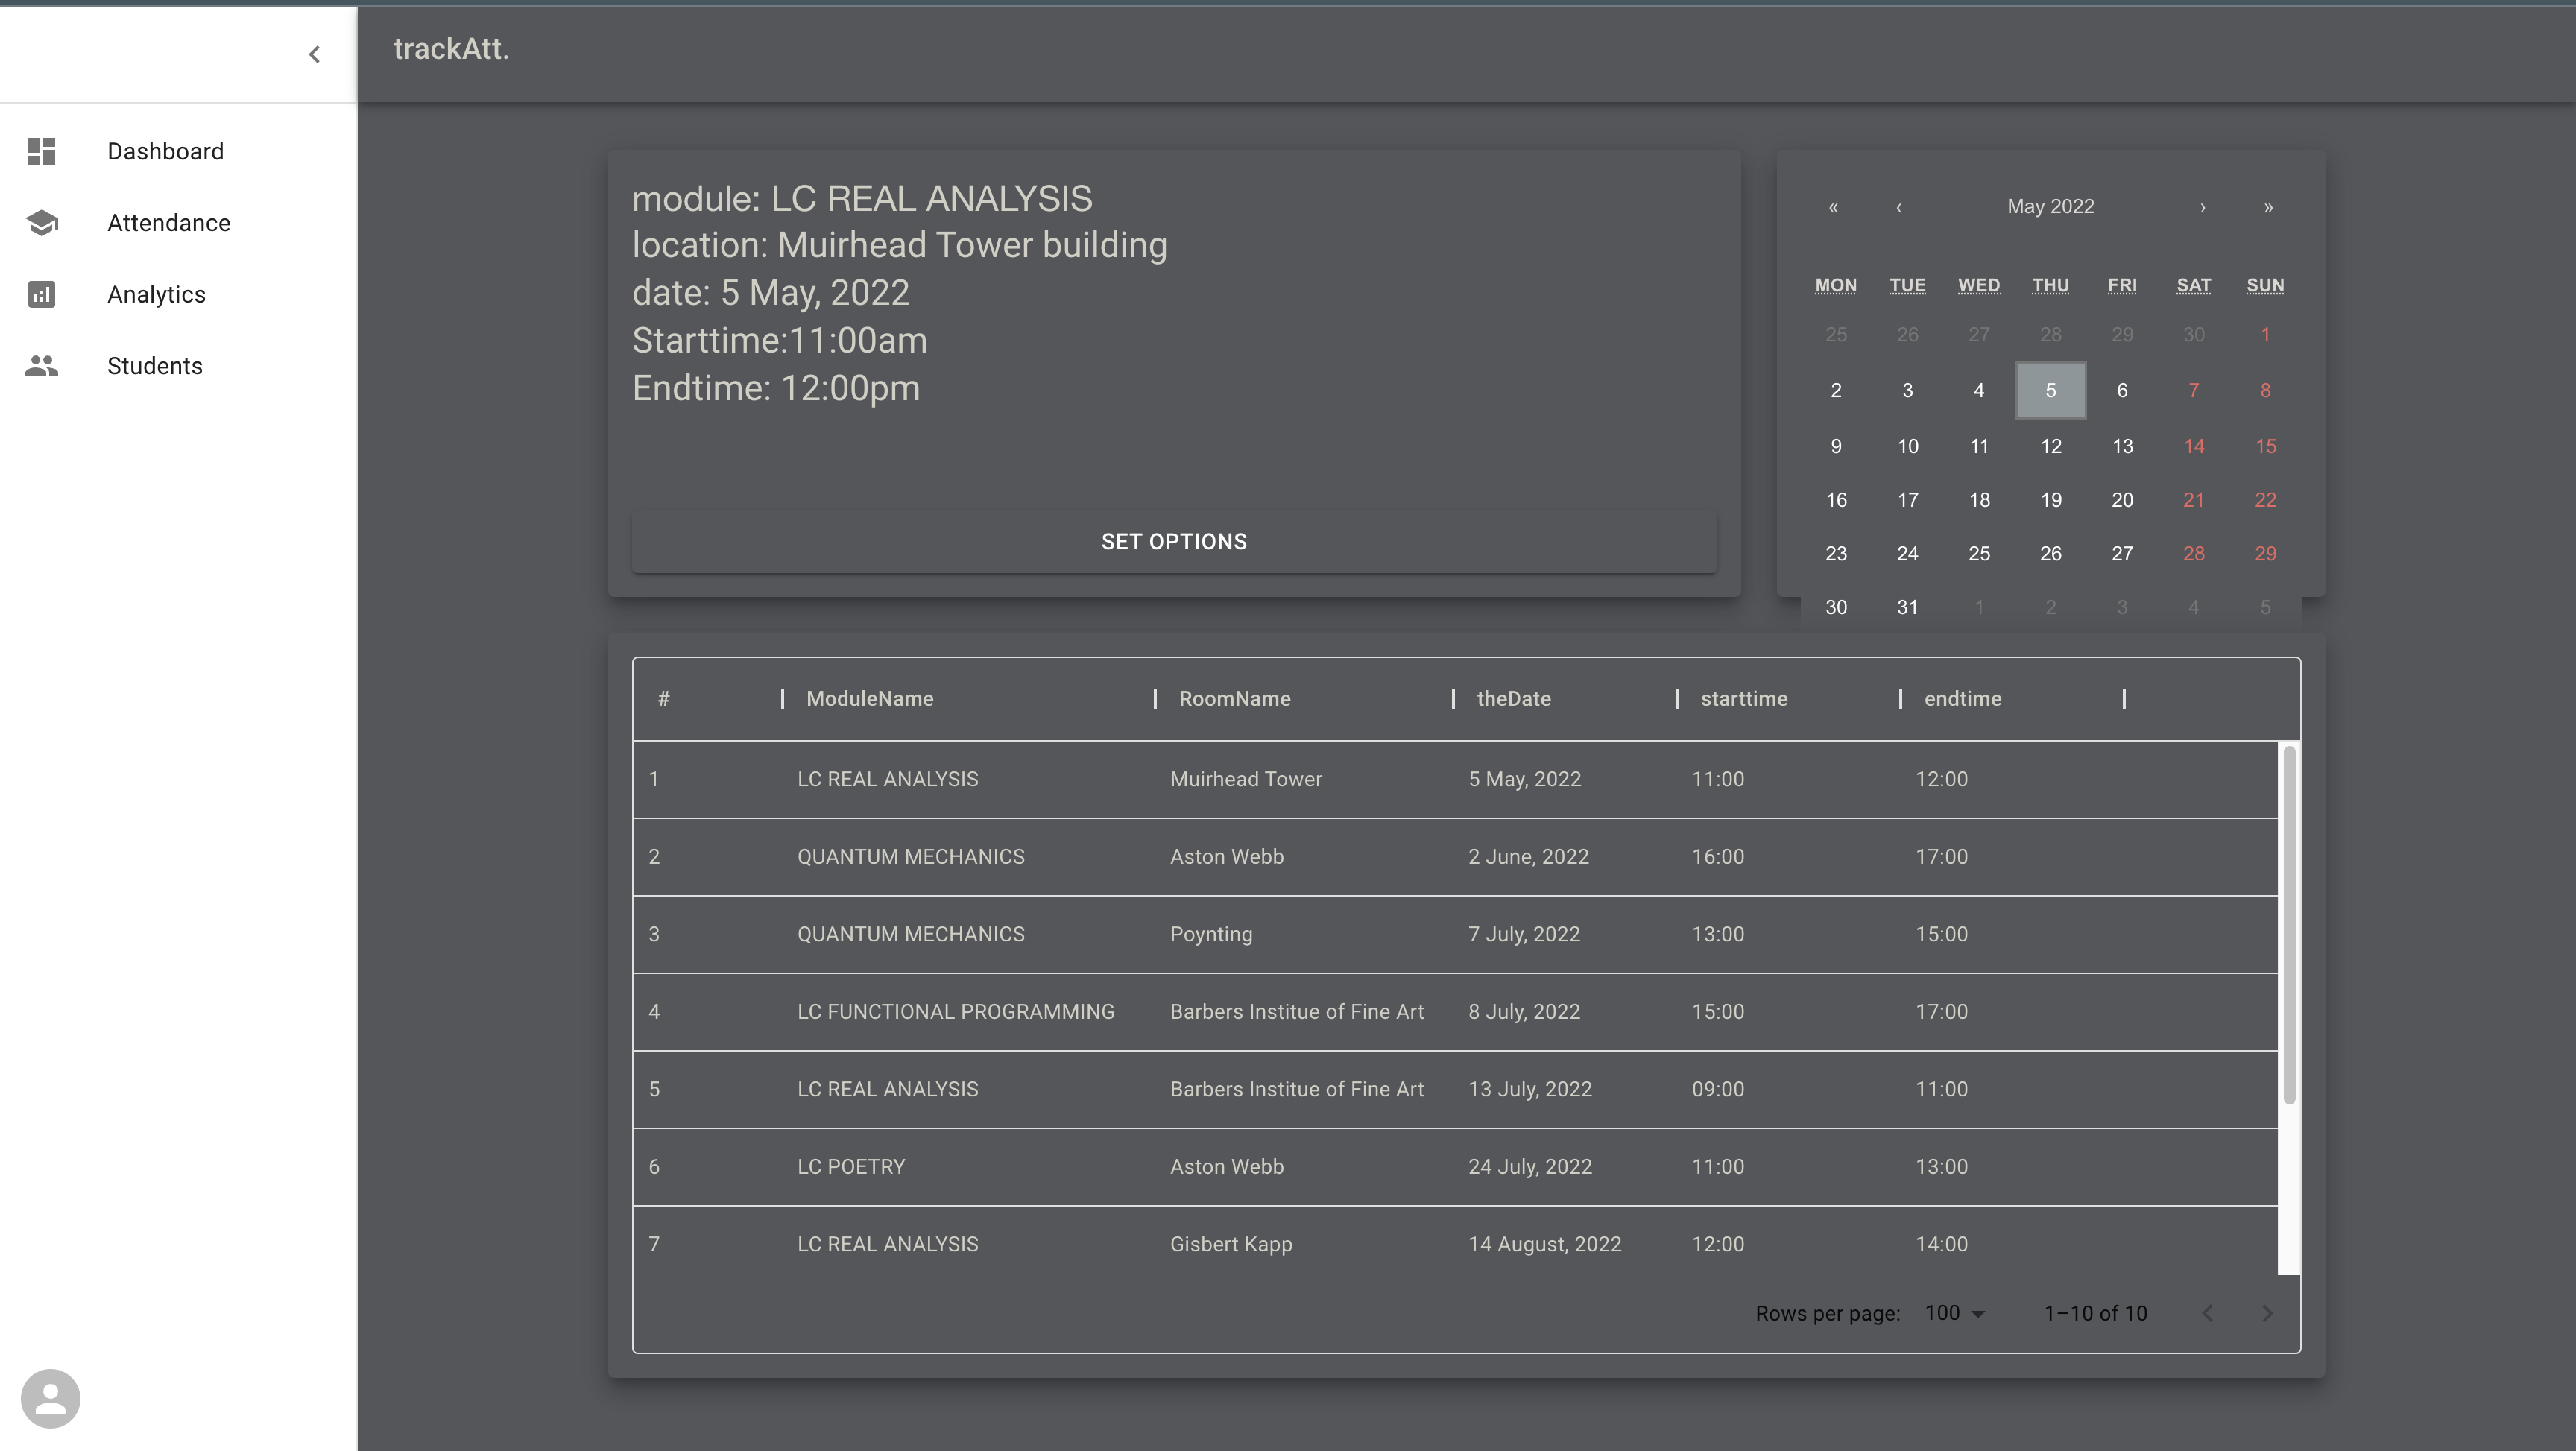
\includegraphics[scale=0.135]{Design & Implementation/images/Dashboard.png}
  \caption{Dashboard/Main page.}
\end{figure}
The main page consists of the EventView at the top left, the CalendarView at the top right and the EventList at the bottom.The functions of these views are:
\begin{itemize}
  \item CalendarView: A date picker that selects the date and sends a request to the server for an event on that date. The default date is the current date at that moment.
  \item EventView: it displays an events information if there is an event on the date requested by the Calendar. It also has a "Set options" button that allows the administrator/lecturer to choose tracking methods and options by redirecting to the Attendance page. 
  \item EventList: it displays a list of future events that the lecturer has.
\end{itemize}
Clicking the "trackAtt." header takes you to the main page.
\subsubsection{Attendance page}
\begin{figure}[ht!]
  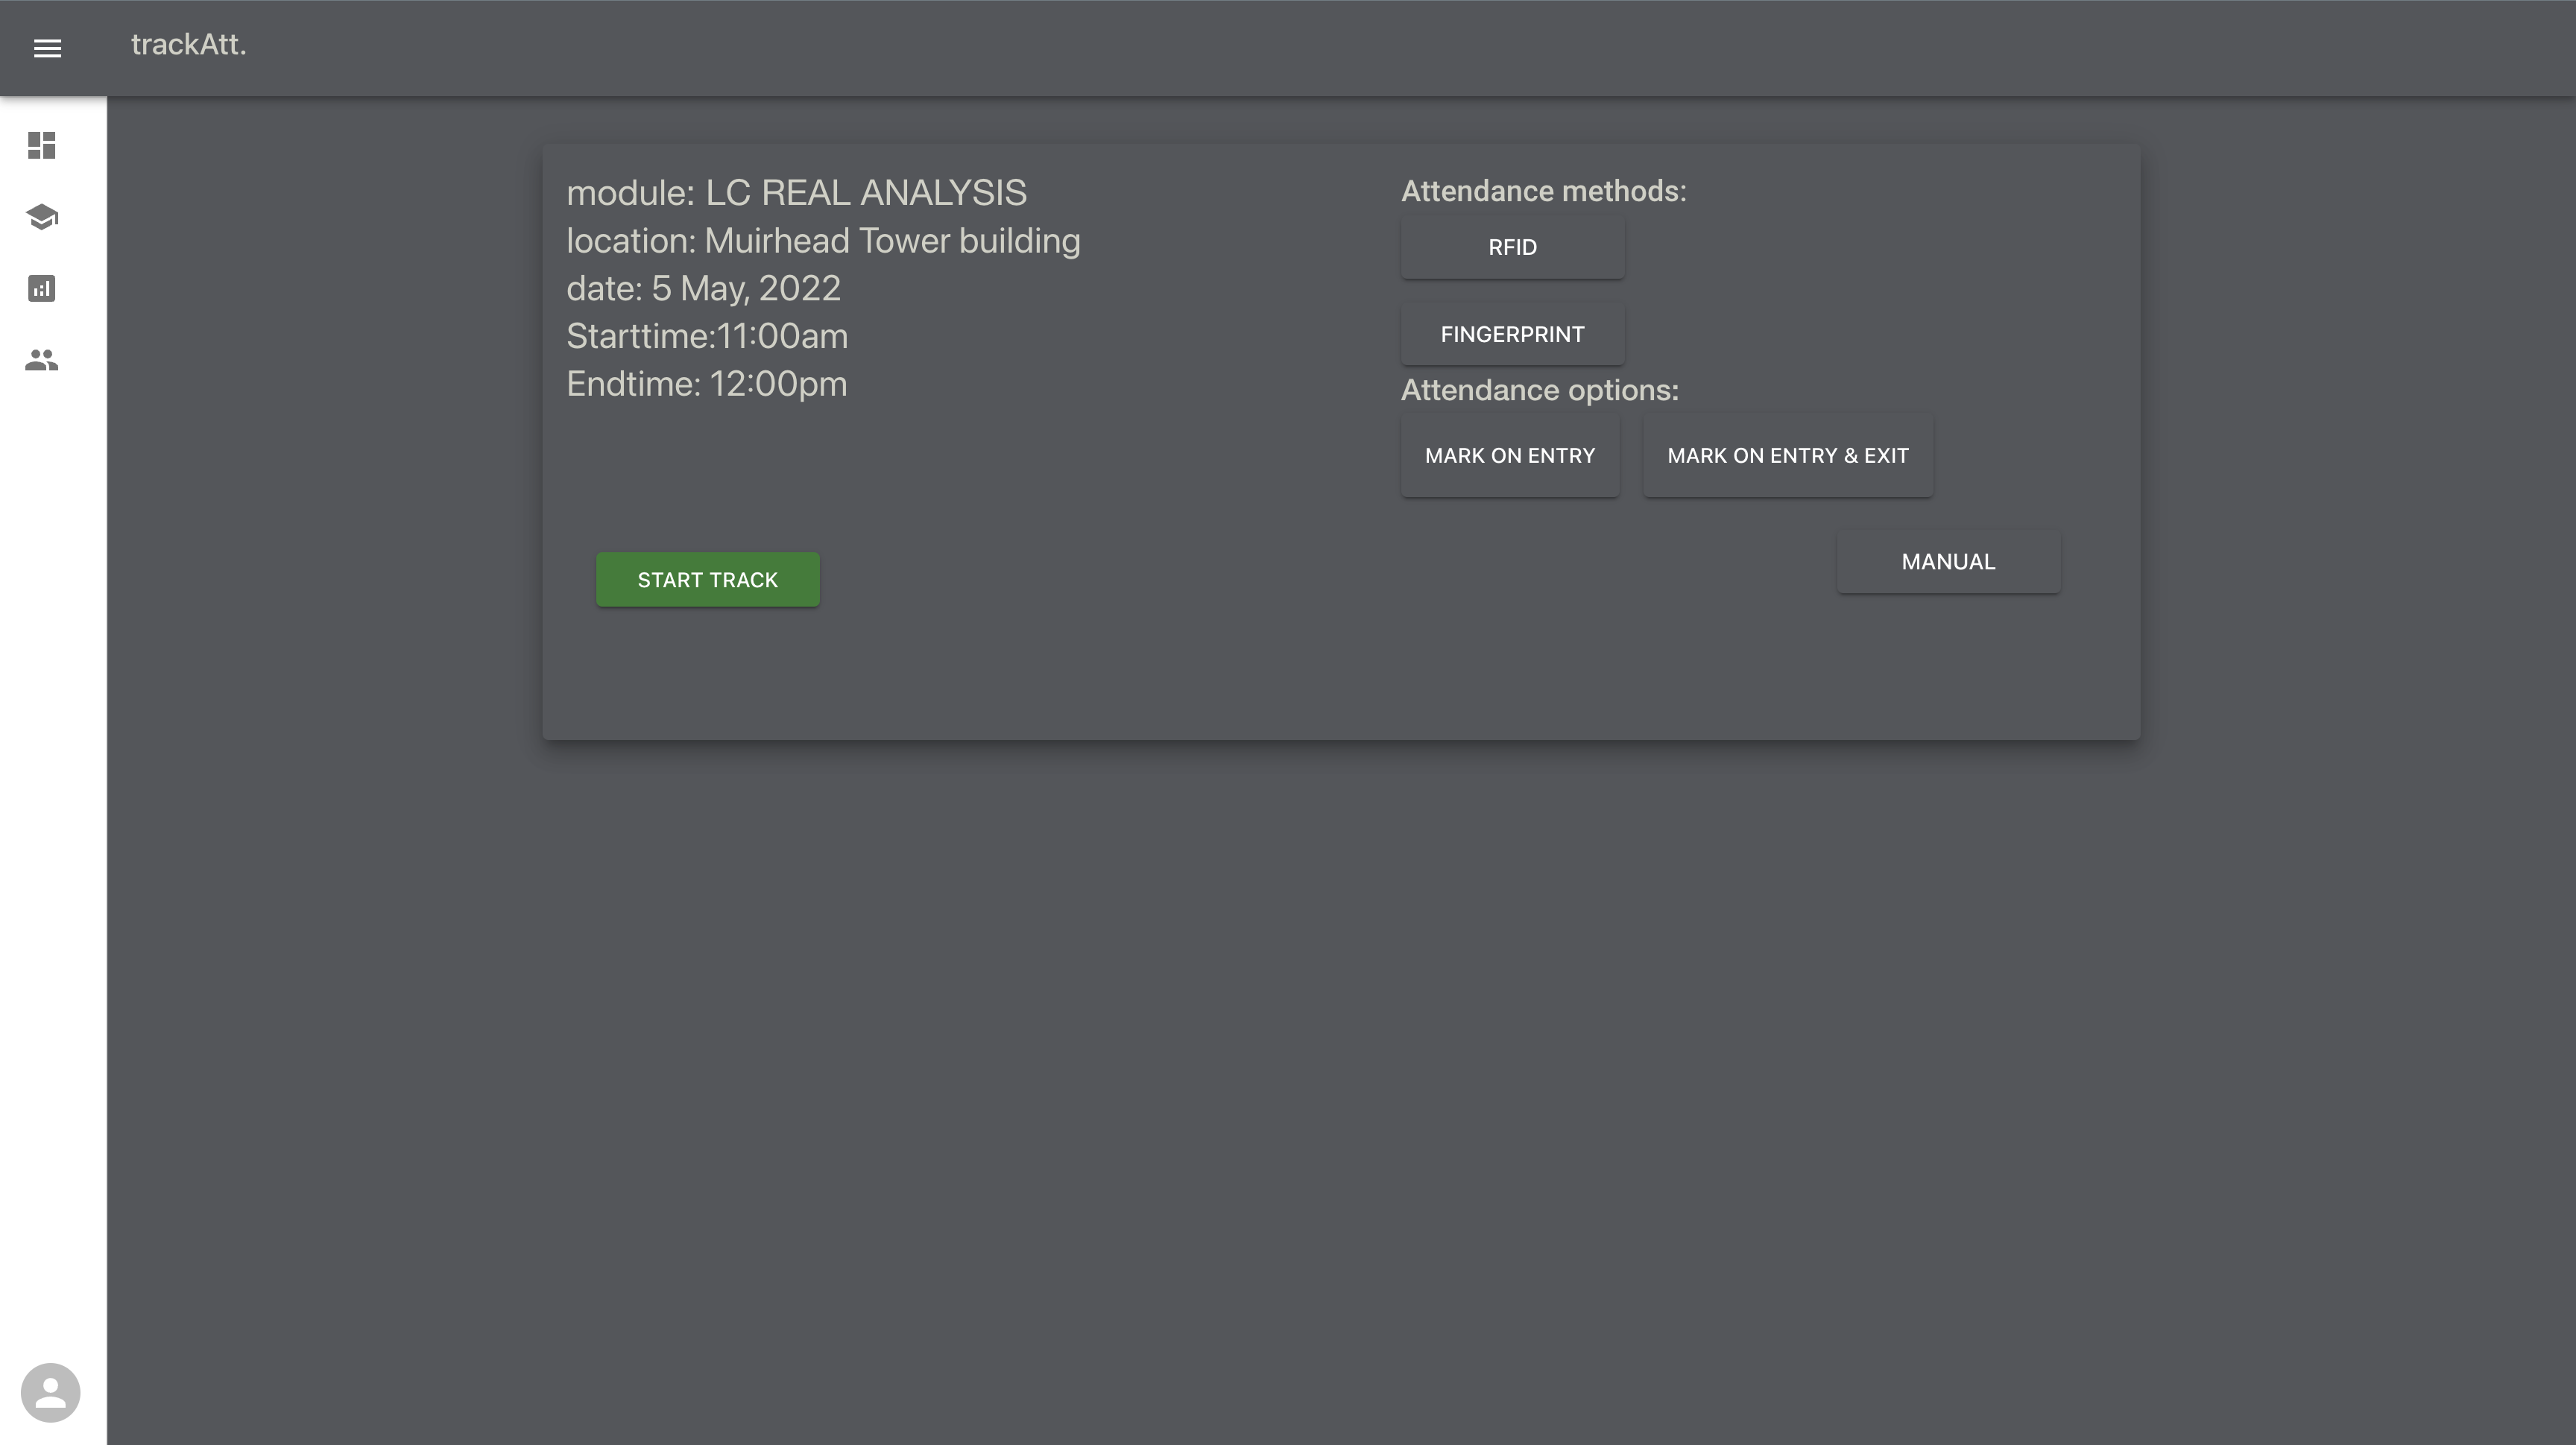
\includegraphics[scale=0.135]{Design & Implementation/images/Attendance.png}
  \caption{Attendance page.}
\end{figure}
The attendance page is mainly gotten to by the "Set options" button of the EventView, if directed to by the dashboard, it should show a list of events to track based on a picker. I couldn't develop this due to time. The main components of the Attendance page are the EventView but without a set options button. Attendance methods with RFID and fingerprint buttons, Attendance options with "mark only Entry" and "mark both Entry and Exit", a "Manual" button and a "Start Track" button. The functions of these components are;

\begin{itemize}
  \item EventView: displays information on the Event requested before by the CalendarView, gets a JSON response from the server and formats the 
  \item Attendance Methods: One method is chosen here, Either the Fingerprint method, the RFID method or the Manual method. Clicking on the fingerprint button sets the JM-101 module as the chosen method for tracking attendance while, clicking on the RFID button sets the RC522 module as the chosen method for tracking attendance, the manual method is for a worst-case scenario where the Raspberry-pi can not track attendance and the teacher knowing each students by name can tick who is absent or present, clicking the button redirects to the Manual page. 
  \item Attendance Options: just like the Attendance Methods just one option can be used, clicking the "mark on entry" button sets the chosen tracking method to track only when the user scans at the beginning of the event while, "mark on both entry \& exit" requires the user to scan at the beginning and end of the event.
  \item Start Track button: starts the tracking method with the attendance options chosen and also redirects to the "InProgress" page.  
\end{itemize}

\newacronym{JSON}{$JSON$}{JavaScript Object Notation}
\glsadd{JSON}

\subsubsection{InProgress page}
The InProgress page comprises of a timer, a "Stop Track" button and a UserView that shows a list of Students that are required for that module. initially I thought of displaying a list that refreshes every minute but did not because I thought this would be quite distractive to the admin while he's using the system for a different action. 


\subsubsection{Analytics page}
The Analytics page contains the Attendance status of the event that was tracked and a pie chart diagram that shows the percentage of student who attended that session. 

\subsubsection{Students page}
The Students page contains the whole list of students in the database.

\subsubsection{Manual page}
The Manual page displays a list of students each row has a checkbox that can be checked, If checked and submitted the students checked will be registered as present.



\subsection{Web server - NodeJS}
NodeJS is really good at handling simultaneous connections. In this project we're sending and receiving data from the database, the flask server and the front-end and sometimes they are concurrently. Tedious is a package that allows the implementation of TDS which is a protocol used to interact with SQL server, this allows me interact with the azure database.
The reason express is used in my project is to mount a middleware at the router-level, this allows me to handle multiple request and responses to multiple end-points with one single mounted root path. 

using the mvc architecture for developing the backend the controller attendanceController.js handles the logic of
These are the major requests and responses handled by the express middleware;
\begin{itemize}
    \item receiveDate: a POST request that sets the date received from the client
    \item sendEvent: a GET request that runs a query to the database that gets all details of an event on a specific date and sends a \gls{JSON} response to the client
    \item sendEventList: a GET request that queries the database that for a list of events which is sent to the client and displayed on the EventList
    \item startTrack: a POST request that gets an Object that consists of the tracking method and option chosen and sends a POST request to the Flask server that runs a script to that start the method chosen
    \item stopTrack: a POST request that checks the method running based on a glob§al variable that was initially set when startTrack was called and sends a POST request to the Flask server endpoint to stop the process
    \item showAttendanceList: a POST request that queries the database for students taking a module based on a classID value that's already been set for the current Event, this returns a response that sends a table containing who was present and absent(status)
    \item showAttendanceListWithoutStatus: a GET request that returns students taking a module based on a classID value
    \item showStudentList: a GET request that returns a list of students taking the current module that is being tracked
    \item showManualAttlist: a GET request similar to the showStudentList but the response is formatted in the front-end
    \item calculateAttendance: a GET request that returns the number of students who are present and absent, this sent to the front-end makes up the pie-chart
    \item addToAttManually: a POST request that adds users from an array gotten from the front-end.
\end{itemize}



\newacronym{TDS}{$TDS$}{Tabular Data Stream}
\glsadd{TDS}
\subsection{Raspberry pi}
I focused on writing a script for the RFID to read information from the RFID tags, when I finished that, I wrote a script to 
I researched on python libraries for RFID
At first I wanted to call each python scripts from the web server but I ran into a series of errors coming from Raspberry pi not being able to grant access for that, and then I found out how to use flask and I came up with the idea of running these scripts from a http endpoint of the flask server.
\subsubsection{fingerprint}
The python Library used was 
At first I was thinking of 
how I used the fingerprint with its flaws

\subsection{Flask}
A major reason why I chose to use flask is because it creates a local server in python, so I don't have to run python scripts in a different language or use an external framework for this.
These are the major requests and responses handled by the flask functions and endpoint.



\subsection{Database}
The database was difficult and complex because of the relationships between different tables, I spent 60\% of my time updating it to fit other parts of the project. I needed it to be hosted on the internet to access it on multiple devices, raspberry and my development computer, At first I used a local MySQL database on my computer but had an issue hosting this on the internet, I switched to Azure because it offered a lot more of other cloud computing services. I created the student table with:

\begin{figure}[ht]
  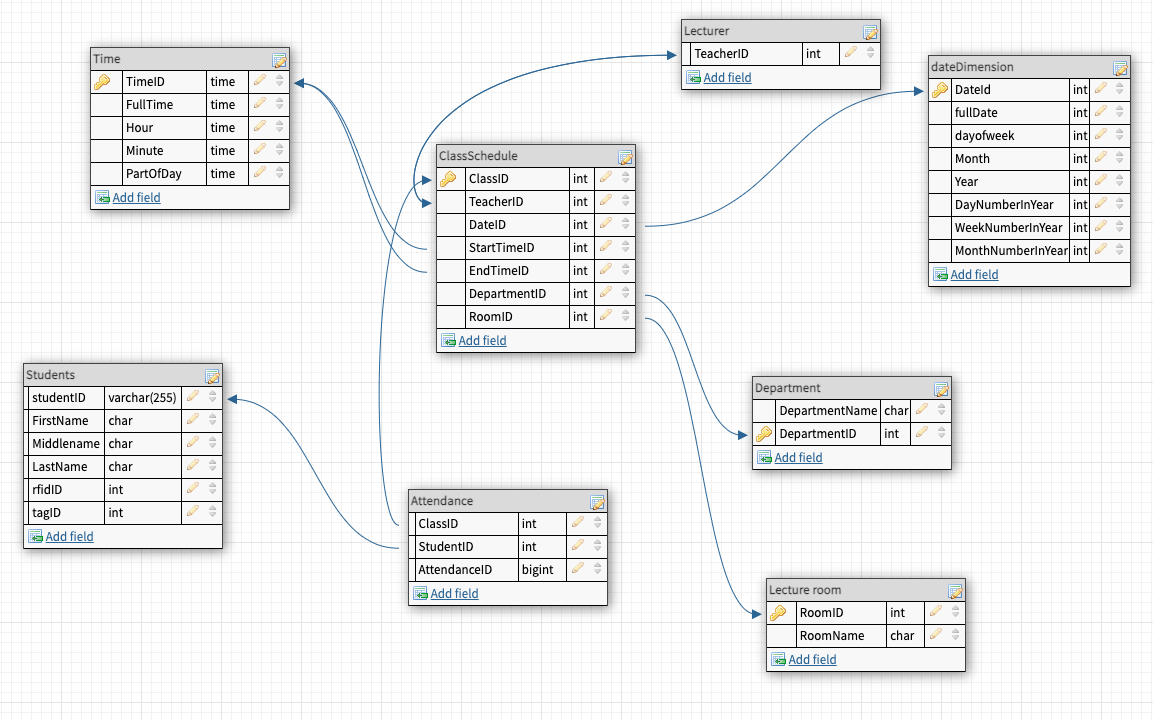
\includegraphics[scale=0.4]{Design & Implementation/images/database_design.png}
  \caption{database design}
\end{figure}

\chapter{Evaluation \& Discussion}
As earlier stated in the Introduction, certain criteria need to be adopted for an evaluation of this project.
\section{Evaluation}
The criteria includes the suitability to track attendance with any of the referred methods, the efficiency in handling the exceptions of unavailable internet or database connection and the ability to show results based on each attendance class.
\subsubsection{Features not implemented \& Limitations}
The system uses just two methods of tracking attendance for now and only one is used at a time. Most of the features that were not implemented was as a result of time and its irrelevance to the aims of the projects. Some of the concepts that could be implemented include;
\begin{itemize}
\item A checker to see if the student has already been added to the database, this would not take much time to be executed.
\item The design of the flask server  The flask server should not be used for production, as it is not designed to be stable, efficient or secure. It does not support all the features of a HTTP server
\item The implementation of the sign-in page and the login page which was not done.
\item The hosting of the NodeJS web server which was not hosted on the internet. The database was the only component of this system that was hosted because its resources were shared between the node webserver and the raspberry pi
\item The implementation of a website page that adds users to the database with their RFID userID values and their fingerprint
\item The system was not implemented to work asynchronously for separate lecturers although a database table with dummy data set for lecturers was established.
\item The system is not designed to concurrently run the implemented attendance methods.
\item Though the database and internet handler works there are some cases where a connection to the web server is limited. This might cause the system not to function effectively as each system can not communicate properly. The test for both handlers might be limited: the system might not function in certain circumstances. This is where the maintenance stage comes into place in agile development.
\end{itemize} 
\subsection{Challenges faced}
Having no knowledge of JavaScript it was an issue learning the concept of React and Node, and no idea of how embedded devices communicate with each other. I had no idea of SQL at the beginning and had to learn the syntax. I had to develop three different systems independently for a certain period and integrate them together.
\subsection{Skills \& Lessons learnt}
There are a great deal of implementations required on a webpage. I went with the requirements for the project based on the time given. Initially having no idea of the web development cycle, focus was centred on irrelevant actions like authentication and style of UI. In the development most of the bugs come from missing out specific variables that are passed as JSON files between systems. A debugging system with a record on variables used would be efficient. A great deal of knowledge about methods embedded devices use to communicate between each other was learned. Valuable concepts and skills such as Latex, Python, JavaScript and SQL were acquired.
\section{Results}
To test this system a dummy dataset was created for the database. The database was used to give an identity to the RFID tag or an individual's fingerprint. A noteworthy and significant aspect of this work is the ability for the administrator to have remote access to the flask server therefore being able to start attendance for the system from anywhere. The system solves all the issues raised in the Introduction. Additionally, the system can be adapted for other functions, such as attendance monitoring in work places. A JUnit or a similar software for this system was not used because it was difficult to test the whole system design. Furthermore, Postman was successfully used to test the API that was created.
\subsection*{Test for handling Database connection}
The test was conducted by pausing the azure database and running the python script solely: without it being called from the flask server. Pausing the database seemed to be a way to test this as it represents objectively, the errors obtained if there was a different cause in the communication between the database and the raspberry pi. The python script seemed to catch and handle the exception by scanning attendance, saving the scanned details in a file, validating and uploading the details from the file when the database was started. As was stated in the Limitations, there might be other factors to be considered to be caught but based on the requirements it works quite well.
 
\subsection*{Test for handling Internet connection}
This was conducted by running the internet handler script\textsuperscript{\ref{internet handler}} separately while switching off the WiFi. This worked effectively based on the constraints given. It caught the exception and handled it by running the offline tracking code. There might be some exceptions that were not handled. Testing the script with the system would require all parts of the system to be hosted on the internet. Due to time at hand this was not possible.
 
\subsection*{Tracking with different choices and attendance methods}
Tracking with different choices and methods was carried out in the course of research. This is the testing stage in the agile development work cycle. It involves testing, by running the system on the expected workflow that was discussed in the Design \& Implementation chapter.
\subsubsection*{fingerprint attendance}
The experiment involves raw fingerprints(from people) already enrolled into the database. For simplicity, the sum of three students used to represent a class. Their fingerprints were given the names: \textbf{A}, \textbf{B}, \textbf{C}. The two attendance choices were tested with the following cases; 
\begin{itemize}
 \item \textbf{mark on Entry only}: \textbf{A} was scanned twice to test both the green and blue responses. This was attained. However, a different fingerprint not enrolled in the module was scanned and produced the red LED response. Similarly, another that was not registered in the database was also scanned and produced the same result. \textbf{B} was scanned but \textbf{C} was not. This produced \textbf{A} and \textbf{B} present but \textbf{C} was absent.
 \item \textbf{mark both Entry and Exit}: \textbf{A} was scanned once to test if it was going to be present on the attendance list. \textbf{B} was scanned thrice to test if it will be present on the attendance list and get the LED responses expected. A green LED response was given for the first two scans. The second response was distinct with respect to the number of times it blinked. A blue LED was given for the third scan. \textbf{C} was not scanned. A different fingerprint was scanned producing a red LED response. The result at the end was, \textbf{B} present. \textbf{A} and \textbf{C} were not.
\end{itemize}
 
\subsubsection*{rfid attendance}
The \gls{RFID} tags were tested with \gls{RFID} tags already enrolled into the database. The class also contained the sum of three students. \gls{RFID} tags are given names: \textbf{A}, \textbf{B}, \textbf{C} for clarity in the explanation. The two attendance choices were tested with the following cases.
\begin{itemize}
 \item \textbf{mark on Entry only}: \textbf{A} was scanned twice to test both the green and blue responses. This was attained. A different tag not enrolled in the module was scanned. This produced the red LED response. Similarly, another tag that was not enrolled in the database was also scanned and produced the same result. \textbf{B} was scanned but \textbf{C} was not. This produced \textbf{A} and \textbf{B} present but \textbf{C} was absent.
 \item \textbf{mark both Entry and Exit}: tag \textbf{A} was scanned once to test if it was going to be present on the attendance list. \textbf{B} was scanned thrice to test if it will be present on the attendance list and to obtain the LED responses. A green LED response was given for the first two scans. The second response was distinct with respect to the number of times it blinked. A blue LED was given for the third scan. \textbf{C} was not scanned. A different tag  not enrolled was scanned producing a red LED response. The result at the end was, \textbf{B} present. \textbf{A} and \textbf{C} were not.
\end{itemize}
 
\subsubsection*{manual attendance}
The manual attendance was tested by running it on the systems workflow but clicking the manual button in the Attendance page. Three students were used. Two were clicked and in the Analytics page, those two were present while the other was not.

 
\section{Discussion and Future Improvements}
Overall, this project achieved its aim of implementing an Attendance monitoring system that monitors attendance with the use of RFID and fingerprint method while handling an inefficient internet connectivity. However, the uniqueness of this system can be extended by adding/integrating more tracking methods for different scenarios this will make for a more versatile system. Additionally, by incorporating A QR code method that uses geo-location on the mobile application and checks location before scanning QR code, the system could be further enhanced.  As much as RFID has a simpler implementation, it comes with a lot of limitations. It is easy to fool the system. However, in the near-future,  having a virtual NFC card just like bank cards in phones will be way more safer with respect to the system.The timer on the website along with the allocated time from the database will be used to validate how long the class was held among other things. Having all these methods run concurrently, would increase efficiency in terms of speed and flexibility as well as 
having multiple administrators use this system asynchronously. An AI based recommendation could be sent to lecturers on what attendance tracking methods to be used based on the circumstances of the event. More response systems other than the LED signals could be integrated. However, to really know and understand the outcome of each reading, an LED screen with the name of the student and a sound for each outcome could be incorporated. Another concept would be integrating this into the canvas website used in schools in the UK. This would also help centralise all the data that can be viewed by the student. An adaptation of a microcontroller for this system could prove cost-effective on a long-term basis.

 
 
 


\chapter{Conclusions}
The dissertation presented a new solution for attendance monitoring using other perspectives to address the inefficiencies prevalent in existing systems. It also fills the gap found in the literature on monitoring systems. 

While reviewing the literature and noting their central argument, it was observed that most of the literature sought to tackle attendance with one solution. Which is to improve the efficiency of the attendance method used. Though there are major solutions that address the argument, they seem to solve this argument in one perspective. The perspective that is advanced is one that enhances the efficiency of these methods against the background of the circumstances it is monitoring. The project is thus a combination of the methods stated in some of the literatures and a novel method of enhancing their efficiency. The project aimed to monitor attendance with multiple methods and also handle unreliable network lapses from the database or the internet. 

In view of the above, a system that monitors attendance with a web application to interact with the process was designed. A manual method website that enables the administrator to click students present was incorporated. While a \gls{RFID} method and a fingerprint method was also used. Each component of the system communicates with each other via a network. This offers an advantage by enabling the administrator to remotely access the web application from anywhere.

A dummy dataset was therefore used to test the system. The dataset was used in the database and the database was used to enrol the \gls{RFID} tags and fingerprints. The project was able to monitor attendance for each event, monitoring attendance with the \gls{RFID}, fingerprint or manually on the website. The system worked perfectly as tracking based on entry or entry and exit was achieved. The system is therefore recommended for adaptation for use by the University of Birmingham.

As much as the project answers the research questions and its aims, there were limitations due to the constraints of time and resources. The major limitations include that posed by the implementation of an authentication page. As stated in the Background\textsuperscript{\ref{authentication}}, a web application needs authentication to supply the resources to the right person. The system is not designed to function asynchronously for seperate lecturers. In a real world scenario, there are multiple administrators of this system and they will need to monitor attendance separately. An option to run some of these methods concurrently would improve the speed and flexibility of this system.

Nonetheless, the next step would be to create a mobile application that tracks attendance using a QR code. The website will display a generated QR code when the QR code method button is clicked. The mobile application checks the location of students before scanning the QR code. The mobile application also has a virtual card that functions as an NFC tag to track attendance. This is a way to provide security and an improvement from the RFID tag which is susceptible to attendance by proxy. The next step would be to make all the designed methods run concurrently so as to make it more flexible. The analytics page would have a list of the dates that attendance has been monitored and from this list one would be able to see the attendance status of that event. The login/signup page would be created and authenticated using the lecturer table in the database.



% \include{chapter6/ch6}



%% APPENDICES %%
\appendix
\chapter{First Appendix}
\vspace*{-0.3in}
\begin{figure}[hb!]
\begin{center}
% \makebox[\textwidth][c]{\includegraphics[width=1\textwidth]{appendix/images/}}
\end{center}
\caption{Again, the example graph.}
\end{figure}


%\include{appendix2/appendix2}

%% BACKMATTER %%
% The pages inside of backmatter are in Arabic numerals and the chapters will not have numeration
\backmatter

% BIBLIOGRAPHY WITH BIBTEX %
%*******************************************************
% Bibliography
%*******************************************************
\cleardoublepage
\phantomsection
\addcontentsline{toc}{part}{References}
\printbibliography[title=References]
\nocite{*}
\vspace{2.5cm}
\begin{Large}Websites consulted\end{Large}
\begin{itemize}
\item Wikipedia -- \url{www.wikipedia.org}
\end{itemize}


% All the sources are described in a file named bibliography.bib
% if you want to cite one in the text:
% \citep{label}
% In order to update the bibliography you have to execute:
% bibtex main (without ".tex")

% INDEX %
\cleardoublepage
% To help hyperref to jump to the correct page
\phantomsection
% To add the Index in the table of contents
\addcontentsline{toc}{chapter}{Index}
% Prints the Index
\printindex
% To add an item in it, write the \index{WORD} after the word to highlight:
% WORD\index{WORD}
% In order to update the Index you have to execute:
% makeindex main (without ".tex")

% A typical session involving a bibliography, an index and so on would require:
% pdflatex main
% makeindex -s main.ist -t main.alg -o main.acr main.acn
% makeindex -s main.ist -t main.glg -o main.gls main.glo
% bibtex main
% pdflatex main
% pdflatex main
% makeindex main
% makeindex -s main.ist -t main.alg -o main.acr main.acn
% makeindex -s main.ist -t main.glg -o main.gls main.glo
% pdflatex main
% pdflatex main
\end{document}